\chapter{Design of Integrated Controller and Compliant Power Supply}

In this chapter, we delve into the comprehensive architecture and design of the integrated controller and compliant power supply for USB Power Delivery (USB PD). The primary objective is to elucidate the intricate interplay between the controller and power supply components, ensuring seamless power delivery and compliance with USB PD standards.

The chapter begins with an overview of the system architecture, highlighting the key modules and their interconnections. This includes the power management unit, control logic, communication interfaces, and protection mechanisms. Each module’s role and functionality are discussed in detail, providing a clear understanding of how they contribute to the overall system performance.

Following the architectural overview, the design considerations for each module are explored. This section addresses the critical design parameters, such as efficiency, thermal management, and electromagnetic compatibility (EMC). Special emphasis is placed on the design of the power supply, which must meet stringent USB PD specifications while maintaining high efficiency and reliability.

The chapter also covers the integration challenges and solutions, focusing on the synergy between the controller and power supply. This includes the design of feedback loops, control algorithms, and the implementation of safety features to protect against overvoltage, overcurrent, and thermal runaway conditions. 
\section{Design Objectives}

\begin{enumerate}
\item To design and implement an USB PD 3.1 compliant controller using CMOS Technology.
\item To design and implement an USB PD 3.1 compliant Power Supply using BCD
Technology.
\item To integrate the designed controller and Power Supply.

\end{enumerate}


\section{System Architecture}

\begin{figure}[hbt]
    \centering
    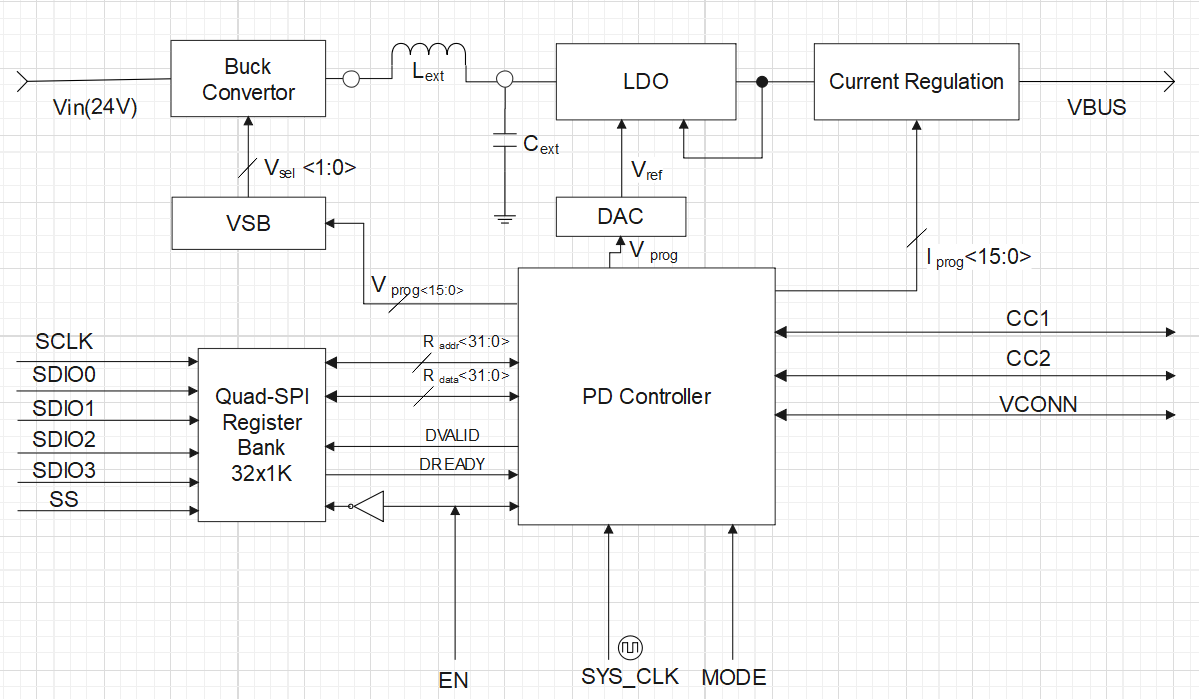
\includegraphics[width=1\linewidth]{Chapter3/BD.png}
    \caption{Architecture of the proposed design}
    \label{fig:bd}
\end{figure}

Figure\ref{fig:bd} illustrates the proposed system architecture for a USB Power Delivery (USB PD) solution. At the core of the design is a Buck Converter that steps down the input voltage (Vin) of 24V to a lower voltage suitable for the system. This is followed by a Low Dropout Regulator (LDO), which further stabilizes the voltage. The Current Regulation block ensures that the output current to the VBUS is controlled and within safe limits. 

Additionally, a Digital-to-Analog Converter (DAC) is used to set the reference voltages for the current regulation, with inputs from ( V\textunderscore {prog} ) and ( I\textunderscore{prog} ). The PD Controller is a critical component that manages the USB PD communication and control, interfacing with the system through serial communication lines (SCLK, SDIO0--SDIO3, SS) and control pins (EN, SYS\textunderscore CLK, MODE). It also connects to the CC1 and CC2 pins for USB PD communication and VCONN for powering the cable.

This integrated design ensures efficient power delivery, precise voltage and current regulation, and compliance with USB PD standards, making it suitable for modern electronic devices requiring reliable power management\cite{st_vbus_control}.

\section{Design of Controller}

“The USB PD Physical Layer consists of a pair of transmitters and receivers that communicate across a single signal wire (CC). All communication is half duplex. The PHY Layer practices collision avoidance to minimize communication errors on the channel"\cite{usb_power_delivery}.

The transmitter performs the following functions:
\begin{enumerate}
    \item Receive packet data from the protocol layer.
    \item Calculate and append a CRC.
    \item Encode the packet data including the CRC (i.e., the payload).
    \item Transmit the Packet including Preamble, \gls{sop}, data, \gls{crc} and \gls{eop} across the channel using \gls{bmc} over CC.
\end{enumerate}
The receiver performs the following functions: 
\begin{enumerate}
    \item Recover the clock and lock onto the Packet from the Preamble.
    \item Detect the \gls{sop}.
    \item Decode the received data including the CRC.
    \item Detect the EOP and validate the CRC: 
    \begin{enumerate}
        \item If the CRC is Valid, deliver the packet data to the protocol layer.
        \item If the CRC is Invalid, flush the received data.
    \end{enumerate}
\end{enumerate}

\subsection{Symbol Encoding }

“With the exception of the Preamble, all communications on the line must be encoded using a line code to maintain a reasonable level of DC-balance and ensure an adequate number of transitions. This encoding simplifies the receiver design and allows for greater flexibility in its implementation. The 4b5b line code will be used, which translates 4-bit data into 5-bit symbols for transmission and converts 5-bit symbols back into 4-bit data for the receiver’s use"\cite{liu2023transient}.

\begin{table}[H]
    \centering
    \caption{4b5b Symbol Encoding Table}
    \begin{tabular}{|c|c|c|c|}
        \hline
        \textbf{Name} & \textbf{4b} & \textbf{5b Symbol} & \textbf{Description} \\
        \hline
        0 & 0000 & 11110 & hex data 0 \\
        1 & 0001 & 01001 & hex data 1 \\
        2 & 0010 & 10100 & hex data 2 \\
        3 & 0011 & 10101 & hex data 3 \\
        4 & 0100 & 01010 & hex data 4 \\
        5 & 0101 & 01011 & hex data 5 \\
        6 & 0110 & 01110 & hex data 6 \\
        7 & 0111 & 01111 & hex data 7 \\
        8 & 1000 & 10010 & hex data 8 \\
        9 & 1001 & 10011 & hex data 9 \\
        A & 1010 & 10110 & hex data A \\
        B & 1011 & 10111 & hex data B \\
        C & 1100 & 11010 & hex data C \\
        D & 1101 & 11011 & hex data D \\
        E & 1110 & 11100 & hex data E \\
        F & 1111 & 11101 & hex data F \\
        \hline
        \textcolor{blue}{Sync-1} & K-code & 11000 & Startsynch \#1 \\
        \textcolor{blue}{Sync-2} & K-code & 10001 & Startsynch \#2 \\
        \textcolor{red}{RST-1} & K-code & 00111 & Hard Reset \#1 \\
        \textcolor{red}{RST-2} & K-code & 11001 & Hard Reset \#2 \\
        \textcolor{blue}{EOP} & K-code & 01101 & EOP End of Packet \\
        \hline
        \textcolor{gray}{Reserved} & \textcolor{gray}{Error} & 00000 & \textcolor{gray}{Shall Not be used} \\
        \textcolor{gray}{Reserved} & \textcolor{gray}{Error} & 00001 & \textcolor{gray}{Shall Not be used} \\
        \textcolor{gray}{Reserved} & \textcolor{gray}{Error} & 00010 & \textcolor{gray}{Shall Not be used} \\
        \textcolor{gray}{Reserved} & \textcolor{gray}{Error} & 00011 & \textcolor{gray}{Shall Not be used} \\
        \textcolor{gray}{Reserved} & \textcolor{gray}{Error} & 00100 & \textcolor{gray}{Shall Not be used} \\
        \textcolor{gray}{Reserved} & \textcolor{gray}{Error} & 00101 & \textcolor{gray}{Shall Not be used} \\
        \textcolor{blue}{Sync-3} & K-code & 00110 & Startsynch \#3 \\
        \textcolor{gray}{Reserved} & \textcolor{gray}{Error} & 01000 & \textcolor{gray}{Shall Not be used} \\
        \textcolor{gray}{Reserved} & \textcolor{gray}{Error} & 01100 & \textcolor{gray}{Shall Not be used} \\
        \textcolor{gray}{Reserved} & \textcolor{gray}{Error} & 10000 & \textcolor{gray}{Shall Not be used} \\
        \textcolor{gray}{Reserved} & \textcolor{gray}{Error} & 11111 & \textcolor{gray}{Shall Not be used} \\
        \hline
    \end{tabular}
    
    \label{tab:4b5b_symbol_encoding}
\end{table}

The 4b5b code provides data encoding along with special symbols. Table\ref{tab:4b5b_symbol_encoding} lists all possibilities of the 4b5b code.

\subsection{Transmitted Bit Ordering}
\begin{figure}
    \centering
    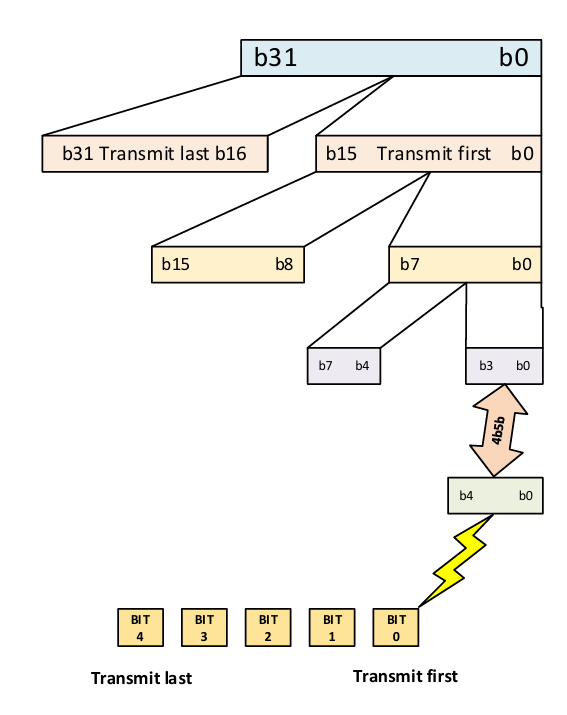
\includegraphics[width=0.5\linewidth]{Chapter3/bit_order.png}
    \caption{Transmit Order for Various Sizes of Data\cite{usb_power_delivery}}
    \label{fig:bit_order}
\end{figure}

The figure\ref{fig:bit_order} illustrates the sequence in which data of different sizes (4 bits, 8 bits, 16 bits, and 32 bits) is transmitted in the CC lines.
\begin{enumerate}
    \item 4-bit Data: The transmission starts with the least significant bit (b0) and proceeds to the most significant bit (b3).
    \item 8-bit Data: The bits are transmitted in order from the least significant bit (b0) to the most significant bit (b7).
    \item 16-bit Data: The transmission begins with the least significant bit (b0) and continues to the most significant bit (b15).
    \item 32-bit Data: The bits are transmitted sequentially from the least significant bit (b0) to the most significant bit (b31).
\end{enumerate}
\subsection{CRC}
\begin{figure}[H]
    \centering
    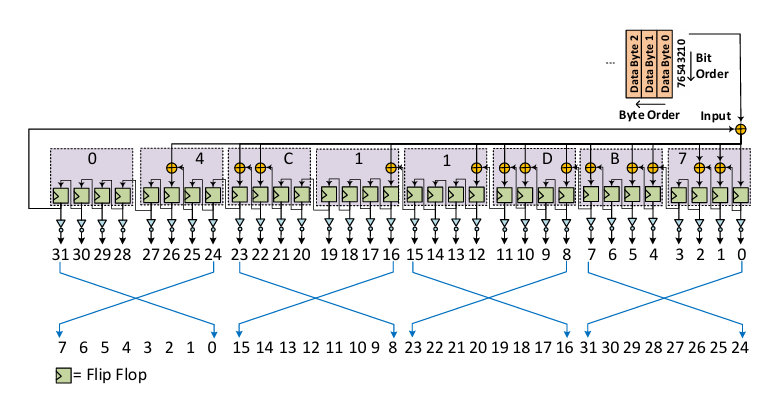
\includegraphics[width=1\linewidth]{crc_ckt.png}
    \caption{CRC 32 generation}
    \label{fig:crc32}
\end{figure}
The Message Header and data are protected by a 32-bit Cyclic Redundancy Check (CRC-32) to ensure data integrity. The CRC-32 polynomial used is 0x04C1\textunderscore1DB7, and the initial value is set to 0xFFFF\textunderscore FFFF. The CRC-32 calculation encompasses all bytes of the payload, excluding any packet framing symbols such as the Preamble, Start of Packet (SOP), and End of Packet (EOP). The calculation starts at byte 0, bit 0, and continues through to bit 7 of each byte in the packet. Once the CRC-32 calculation is complete, the remainder is complemented. The residual value of the CRC-32 is 0xC704\textunderscore DD7B. This inversion of the CRC-32 remainder adds an offset of 0xFFFF\textunderscore FFFF, resulting in a constant CRC-32 residual of 0xC704\textunderscore DD7B at the receiver side. This mechanism ensures that any errors in the data payload can be detected and corrected, maintaining the integrity of the transmitted data\cite{hu2023design}.

\begin{table}[H]
    \centering
        \caption{CRC-32 Mapping}
    \begin{tabular}{|c|c|}
        \hline
        \textbf{CRC-32} & \textbf{Result bit Position in CRC-32 Field} \\
        \hline
        0 & 31 \\
        \hline
        1 & 30 \\
        \hline
        2 & 29 \\
        \hline
        3 & 28 \\
        \hline
        4 & 27 \\
        \hline
        5 & 26 \\
        \hline
        6 & 25 \\
        \hline
        7 & 24 \\
        \hline
        8 & 23 \\
        \hline
        9 & 22 \\
        \hline
        10 & 21 \\
        \hline
        11 & 20 \\
        \hline
        12 & 19 \\
        \hline
        13 & 18 \\
        \hline
        14 & 17 \\
        \hline
        15 & 16 \\
        \hline
        16 & 15 \\
        \hline
        17 & 14 \\
        \hline
        18 & 13 \\
        \hline
        19 & 12 \\
        \hline
        20 & 11 \\
        \hline
        21 & 10 \\
        \hline
        22 & 9 \\
        \hline
        23 & 8 \\
        \hline
        24 & 7 \\
        \hline
        25 & 6 \\
        \hline
        26 & 5 \\
        \hline
        27 & 4 \\
        \hline
        28 & 3 \\
        \hline
        29 & 2 \\
        \hline
        30 & 1 \\
        \hline
        31 & 0 \\
        \hline
    \end{tabular}

    \label{tab:crc32_mapping}
\end{table}

Figure \ref{fig:crc32} and Table \ref{tab:crc32_mapping} show the generation of CRC32 sequence and their mapping. CRC errors, or errors found during the decoding of encoded symbols using the code table, must be handled identically; the message should be discarded, and a GoodCRC message should not be sent. If the CC-line becomes idle at any point while the receiver is processing a packet, the receiver must stop processing and discard the packet, without returning a GoodCRC message.
\subsection{Biphase Mark Coding (BMC) Signaling Scheme}
\begin{figure}
    \centering
    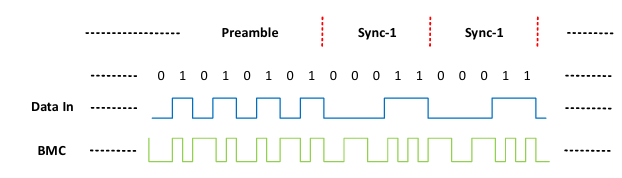
\includegraphics[width=1\linewidth]{Chapter3/bmc_eg.png}
    \caption{Example of BMC signalling}
    \label{fig:bmc_sig}
\end{figure}

“Biphase Mark Coding (BMC) is the physical layer Signaling Scheme for carrying USB Power Delivery Messages.  This 
encoding assumes a dedicated DC connection, identified as the CC wire, which is used for sending PD Messages". 

“Biphase Mark Coding is a version of Manchester coding .  In BMC, there is a transition at the start of every bit time (UI) and there is a second transition in the middle of the UI when a 1 is transmitted.  BMC is effectively DC balanced, (each 1 is DC balanced and two successive zeroes are DC balanced, regardless of the number of intervening 1’s).  It has bounded disparity (limited to 1 bit over an arbitrary packet, so a very low DC level)"\cite{IEC60958-1}. 

\section{Design of Power Supply}
The power supply design is a critical component of the integrated system, ensuring that the USB Power Delivery (USB PD) controller operates efficiently and reliably. This section delves into the design and implementation of the power supply, which is divided into three key subsections: the Buck Converter, the Low Dropout (LDO) Regulator, and the Current Regulation and VBUS Short Circuit Protection.
\subsection{Buck Converter}
The buck converter is responsible for stepping down the input voltage to a lower, regulated output voltage suitable for the USB PD controller\cite{Guerrero2012}. This subsection details the design considerations and component selection of the buck converter, highlighting its efficiency and performance under various load conditions\cite{billings1999switchmode}.

\begin{figure}[H]
    \centering
    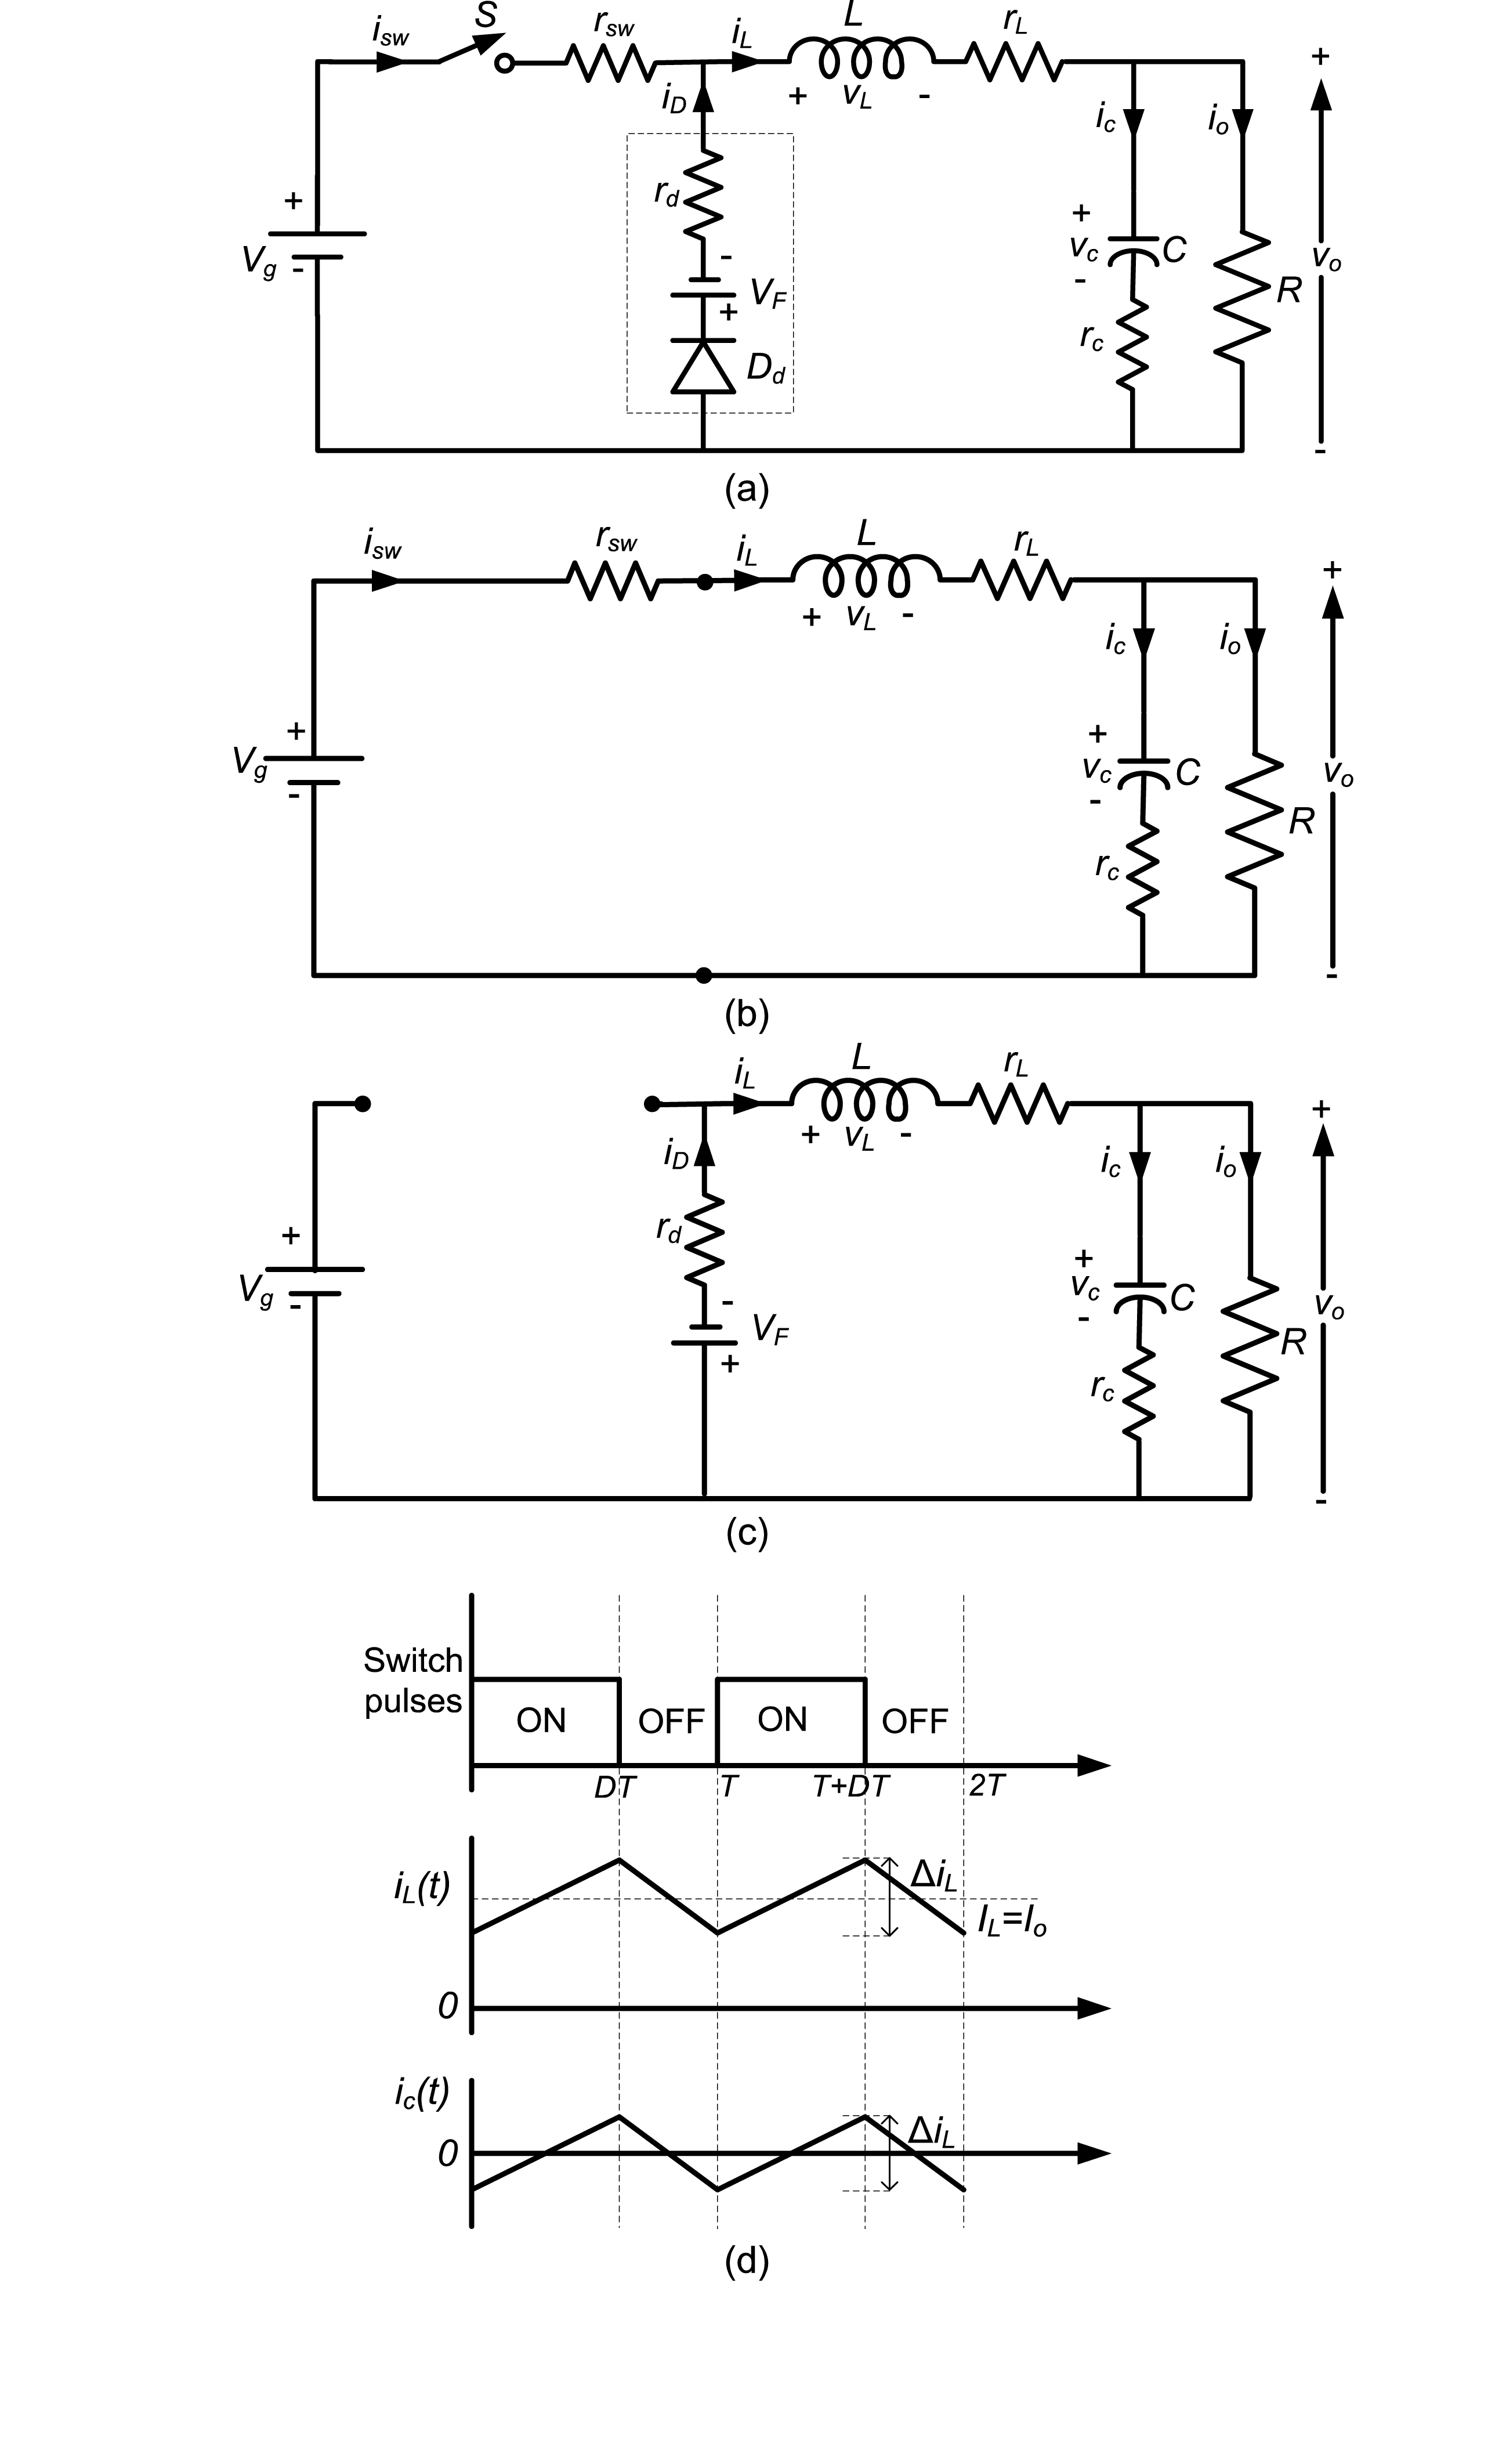
\includegraphics[width=0.75\linewidth]{Chapter3/buck.png}
    \caption{(a) Non-ideal model of Buck Converter (b) switch on equivalent (c) switch-off equivalent (d) I-V waveforms }
    \label{fig:buck_c1}
\end{figure}

The basic circuit of a non-ideal DC-DC buck converter (as seen in Figure \ref{fig:buck_c1}) includes various components with non-ideal characteristics. The converter operates in different modes, and the duty cycle \( D \) is defined as the ratio of the time duration for which the switch is on \( (t_{on}) \) to the total switching period \( (T) \).

\begin{equation}
  \label{c3:eq1}  
  D = \frac{t_{on}}{T}
\end{equation}

Equation \ref{c3:eq1} implies,

\begin{equation}
 D = \frac{t_{\text{on}}}{t_{\text{on}} + t_{\text{off}}} = \frac{t_{\text{on}}}{T} = t_{\text{on}} f_s
 \label{c3:eq2}
\end{equation}

From equation \ref{c3:eq2} , switch on time, \begin{equation}
\label{c3:eq3}
    t_{\text{on}} = {DT}
\end{equation} 

Similarly, switch-off time, 
\begin{equation}
    \label{c3:eq4}
    t_{\text{off}} = (1-{D}){T} = {D'}{T}
\end{equation}

For any DC-DC converter, the inductor design is an important issue \cite{er3}. The inductance \( L \) basically depends upon the operating switching frequency \( f_{SW} \) and desired inductor current ripple \( \Delta i_L \) as the desired inductor current ripple factor (ICRF) such that

\begin{equation}
    \label{c3:eq5}
    ICRF = \frac{\Delta i_L}{I_o} \quad 
\end{equation}



Here, \( I_o \) is the average output current.

In steady-state, during switch-off, \( i_L(t) \) can be written as:

\begin{equation}
   \label{c3:eq6}
   i_L(t) = I_o + \left(\frac{1}{2}\right)\Delta i_L - \left(\frac{t}{T}\right)\Delta i_L  \quad 
\end{equation}



By substituting \( t = T_{off} = T - T_{on} = T(1 - D), V_T = V_o/V_i - 1, V_D = V_f/V_i \) into equation \ref{c3:eq6}, we get

\begin{equation}
    \label{c3:eq7}
     \left(\frac{1}{2}\right)\Delta i_L + V_T + V_D = 0 \quad 
\end{equation}



Substituting equation \ref{c3:eq7} in equation \ref{c3:eq6}

\begin{equation}
\label{c3:eq8}
    L = \left(\frac{V_o}{I_o}\right)\left(\frac{T(1-D)}{\Delta i_L}\right)   \quad 
\end{equation}


where

\[
\begin{aligned}
L &= \text{Inductance}, \\
f_{SW} &= \text{Switching frequency}, \\
ICRF &= \text{Inductor Current Ripple Factor}, \\
I_o &= \text{Average output current}, \\
t &= \text{Time variable}, \\
T &= \text{Period of switching cycle}, \\
D &= \text{Duty cycle of switch-on time to total period}, \\
V_T &= \text{Normalized voltage transfer ratio minus one}, \\
V_D &= \text{Normalized diode forward voltage drop}.
\end{aligned}
\]


\subsection{Low Dropout (LDO) Regulator}
The LDO regulator provides a stable output voltage with minimal ripple, ensuring the smooth operation of sensitive components within the USB PD system\cite{robertson2010thermal}\cite{lee1999ldo}. This subsection covers the design principles, implementation challenges, and performance metrics of the LDO regulator, emphasizing its role in maintaining voltage stability.
\subsubsection{Key Components}

\begin{enumerate}
    \item \textbf{Pass Transistor}: The pass transistor (usually a PNP or PMOS transistor) controls the voltage drop between the input and output\cite{ti_ldo_theory}.
    \item \textbf{Error Amplifier}: The error amplifier compares the output voltage with a reference voltage and adjusts the pass transistor to maintain a constant output voltage\cite{ti_linear_regulators}.
    \item \textbf{Feedback Network}: The feedback network provides a portion of the output voltage back to the error amplifier for regulation\cite{infineon_usb_ccg2}.
\end{enumerate}

\subsubsection{Equations}

\begin{enumerate}
    \item \textbf{Output Voltage}:
    \begin{equation}
\label{c3:eq9}
    V_{out} = V_{ref} \left(1 + \frac{R_1}{R_2}\right)
\end{equation}
  
    \item \textbf{Dropout Voltage}:
    \begin{equation}
\label{c3:eq10}
    VV_{DO} = V_{in} - V_{out}
\end{equation}
    
    \item \textbf{Power Dissipation}:
    \begin{equation}
\label{c3:eq11}
    P_D = (V_{in} - V_{out}) \times I_{out}
\end{equation}
    
    \item \textbf{Efficiency}:
    \begin{equation}
\label{c3:eq12}
    \eta = \frac{V_{out} \times I_{out}}{V_{in} \times I_{in}} \times 100\%
\end{equation}
    
    \item \textbf{Load Regulation}:
    \begin{equation}
\label{c3:eq13}
    \Delta V_{out} = V_{out_{no\_load}} - V_{out_{full\_load}}
\end{equation}
    
    \item \textbf{Line Regulation}:
    \begin{equation}
\label{c3:eq14}
    \Delta V_{out} = V_{out_{min}} - V_{out_{max}}
\end{equation}
    
\end{enumerate}
\subsection{Current regulation and VBUS short circuit protection}

Current regulation and VBUS short circuit protection are essential for safeguarding the USB PD system against overcurrent and short circuit conditions\cite{ti_lm1084}. This subsection discusses the design strategies employed to achieve effective current regulation and protection mechanisms, including the selection of appropriate components and the results of stress tests.

A current mirror is a circuit that copies the current flowing through one active device (transistor) into another, maintaining a constant current regardless of the load. When used in series with a DAC, the current mirror ensures that the output current is regulated and stable.

\subsubsection{Key Components}

\begin{enumerate}
    \item \textbf{Current Mirror}: Typically consists of two transistors (Q1 and Q2) with their bases and emitters connected. The collector current of Q1 sets the reference current, which is mirrored by Q2.
    \item \textbf{DAC}: Converts digital signals into an analog current, which is then regulated by the current mirror.
\end{enumerate}

\subsubsection{Equations}

\begin{enumerate}
   
    \item \textbf{Mirrored Current}:
    \begin{equation}
\label{c3:eq15}
    I_{OUT} = [\beta] \cdot I_{REF}
\end{equation}
    
    In an ideal current mirror, the current through the output transistor (Q2) \(( I_{OUT} \)) is equal to the \(\beta\) times the reference current \(( I_{REF} )\). This means that the current mirror copies the reference current to the output, ensuring a stable and regulated current. \(\beta\) is the ratio of widths of mirrored current transistor to that of reference current transistor\cite{er1}.
    \item \textbf{Voltage Drop Across Transistors}:
    \begin{equation}
\label{c3:eq16}
    V_{CE} = V_{CC} - I_{OUT} \times R_{LOAD}
\end{equation}
    
    This equation calculates the collector-emitter voltage \(( V_{CE} )\) of the output transistor (Q2) in the current mirror. The voltage drop across the transistor is determined by the supply voltage \(( V_{CC} )\), the output current \(( I_{OUT} )\), and the load resistor \(( R_{LOAD} )\). This equation helps in understanding the voltage conditions across the transistor, which is crucial for ensuring proper operation and avoiding saturation\cite{er2}.
\end{enumerate}

This chapter outlines the architecture of the integrated controller and compliant power supply for USB Power Delivery (USB PD). Key modules include the power management unit, control logic, communication interfaces, and protection mechanisms. It discusses critical design parameters such as efficiency, thermal management, and electromagnetic compatibility (EMC). Special emphasis is placed on the power supply design to meet stringent USB PD specifications. Specific design elements like the Buck Converter, Low Dropout (LDO) Regulator, and Current Regulation and VBUS Short Circuit Protection are detailed, highlighting their roles in ensuring efficient and reliable power delivery.
